\documentclass{article}
\usepackage{amsmath}
\usepackage{amssymb}
\usepackage{graphicx}
\graphicspath{ {./images/} }
\usepackage[title]{appendix}
%\usepackage{nips_2018}
\usepackage[a4paper, total={7in, 10in}]{geometry}


\begin{document}
	\title{Solving differential equation by Neural Network}
	\maketitle
	\begin{abstract}
	We formulate ordinary differential equation(ODE) and partial differential equation(PDE) as learning algorithm for neural network. The neural network is trained to satisfy the differential operator and boundary conditions using stochastic gradient descent.
	\end{abstract}


\tableofcontents

\section{Notation}
\begin{enumerate}
	\item Let $\Omega \in \mathbb{N}, \bar{x} \in \Omega, \bar{x}=\{x_1, \dots, x_N\} \in \mathbb{R}^{N}, x_i=\{\frac{i}{N} \}, i=\{1,2 \dots N\}$. Let $j=\{1, \dots, M\}, w \in \mathbb{R}^{1 \times M}, v \in R^{M}$. The output of neural network denotes $Q(v,w,\bar{x})$, $Q=\{Q_1, \dots, Q_N\} \in \mathbb{R}^N$ where $v$ is weight from input to hidden layer, $h$ is hidden unit and $w$ is the weight from hidden to output layer.
	\item The trial solution: $\hat{u}(\bar{x}) = (\hat{u}_{1}, \dots , \hat{u}_{N}) \in \mathbb{R}^{N}$.
	\item The loss function in neural network denotes $E(w,v;\bar{u}(\bar{x})) = \sum_{i=1}^{N}[L(\hat{u})(x_i) - f(x_i)]^{2}$.
	\item Analytic solution of the partial differential equation: $u_{analytic}(x)$

\end{enumerate}
\section{Experiment}
This section presents the detail of implementation and the accuracy of empirical result for numerical examples.

\subsection{Examples for ODE}
\textbf{Problem 1.1}
We would like to find the solution of $u(x)$ for the following equation.
\[\frac{d}{dx}u + \left(x+\frac{1+3x^2}{1+x+x^3}\right)u = x^3 +2x +x^{2}\frac{1+3x^2}{1+x+x^3}\]
with initial conditions $u(0)$ and a boundary condition $u(1)$.
The analytic solution is
\[u_{analytic}(x)=\frac{e ^{-x^2/2}}{1+x+x^3} + x^2\]
In consideration of (\ref{eq:trial_solution}) below, the form of trial solution is taken to be:
\[u_{trial}(\bar{x}) = u(0) + x\bar{u}(w,v,\bar{x})\] 
We look for the solution $u_{trial}$ by minimizing the following error quantity:
\[E(v,w;\bar{u}(\bar{x})) =  \sum_{i=0}^{i=N} \left( \frac{\partial u_{trial} }{\partial x}(x_i)-f(x_i,u_{trial}(x_i))\right)^2\]
where
\[f(x_i,u_{trial}(x_i)) =x_{i}^3 +2x_{i} +x_{i}^{2}\frac{1+3x_{i}^2}{1+x_{i}+x_{i}^3} - u\left(x_{i}+\frac{1+3x_{i}^2}{1+x_{i}+x_{i}^3}\right)\]

\medskip\noindent
In each iteration, we update the weight to be

\begin{equation}
\begin{aligned}
	w_{ij}^{(k+1)} &= w_{ij}^{(k)} - \gamma_{k}*\frac{\partial E}{\partial w_{ij}}(w,v;\hat{u}_i(\bar{x})) \\
	v_{j}^{(k+1)} &= v_{j}^{(k)} - \gamma_{k}*\frac{\partial E}{\partial v_{j}}(w,v;\bar{u}_i(\bar{x})) 
\end{aligned}
\end{equation}

where $\gamma_k$ is the learning rate.

\medskip \noindent
Figure \ref{fig:trial_ode1} displays the actual and computed solution of $u_{trial}(x_i)$ at the grid points.
\begin{figure}
	\centering
	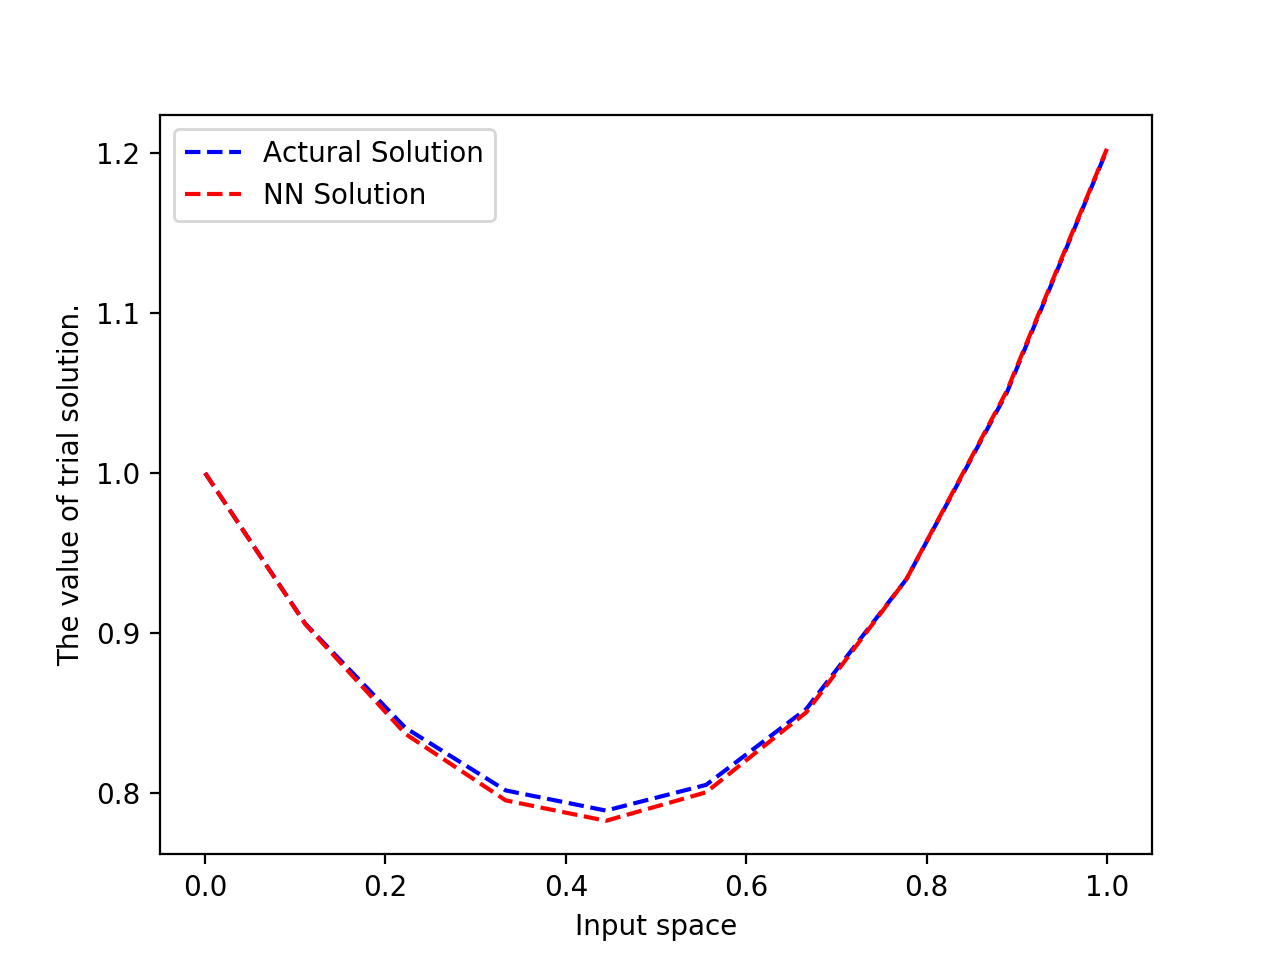
\includegraphics[width=0.5\textwidth]{ode_1.png}
	\caption{The actual and computed solution in problem 1.1. }
	\label{fig:trial_ode1}
\end{figure}

\medskip \noindent
\textbf{Problem 1.2} Given $x_i \in [0,2]$, $1 \leq i \leq N$. We would like to find the solution of $u(x)$ for the following equation.

\[\frac{d}{dx} u + \frac{1}{5} u = e^{\frac{x}{5}}cos(x)\]

\medskip \noindent
The analytic solution is:
\[u_{analytic}(x) = e^{\frac{1}{5}}sin(x) \]
In consideration of (\ref{eq:trial_solution}) below, the form of trial solution is taken to be:
\[u_{trial}(\bar{x}) = u(0) + x\bar{u}(\bar{x})\] with initial condition $u(0)$ and a boundary condition $u(2)$.

\medspace \noindent
Figure \ref{fig:trial_ode2} displays the actual and computed solution of $u _t(x_i)$ corresponding to the domain.

\begin{figure}
	\centering
	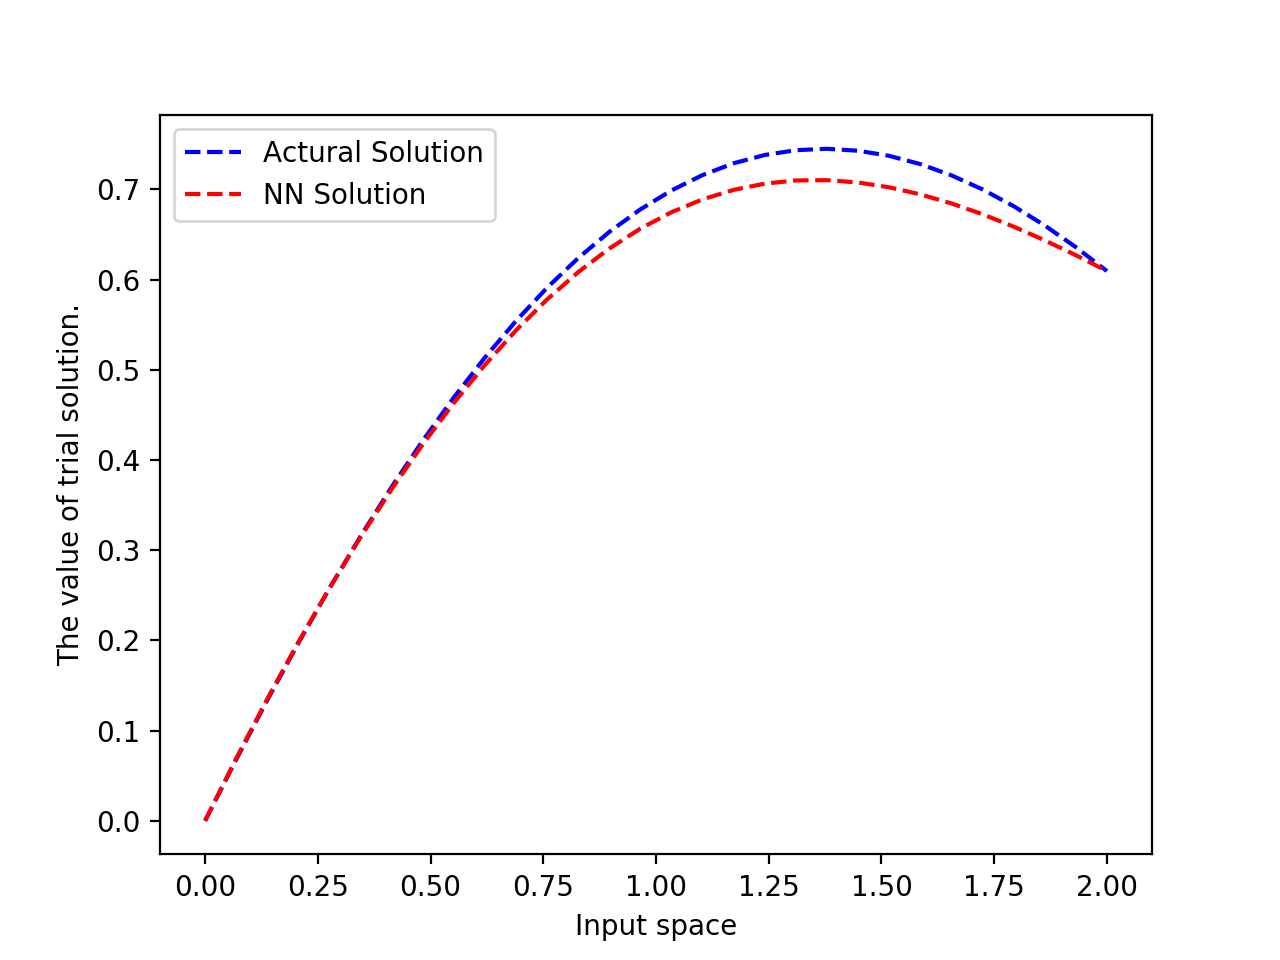
\includegraphics[width=0.5\textwidth]{ode_2.png}
	\caption{The actual and computed solution in problem 1.2. }
	\label{fig:trial_ode2}
\end{figure}

\medskip \noindent
\textbf{Problem 1.3} Given $x_i \in [0,2]$, $1 \leq i \leq N$. We would like to find the solution of $u(x)$ for the following equation.

\[\frac{d^2}{dx^2} u + \frac{1}{5} \frac{d}{dx} u + u= -\frac{1}{5}e^{\frac{x}{5}}cos(x)\]

\medskip \noindent
The analytic solution is:
\[u_{analytic}(x) = e^{\frac{1}{5}}sin(x) \]
In consideration of (\ref{eq:trial_solution}) below, the form of trial solution is taken to be:
\[u_{trial}(\bar{x}) = u(0)(1-\bar{x})+ u(1)\bar{x}+x(1-x_i)\bar{u}(\bar{x})\] with initial conditions $u(0)$ and a boundary condition $u(2)$.

\medspace \noindent
Figure \ref{fig:trial_ode3} displays the actual and computed solution of $u _t(x_i)$ corresponding to the domain.

\begin{figure}
	\centering
	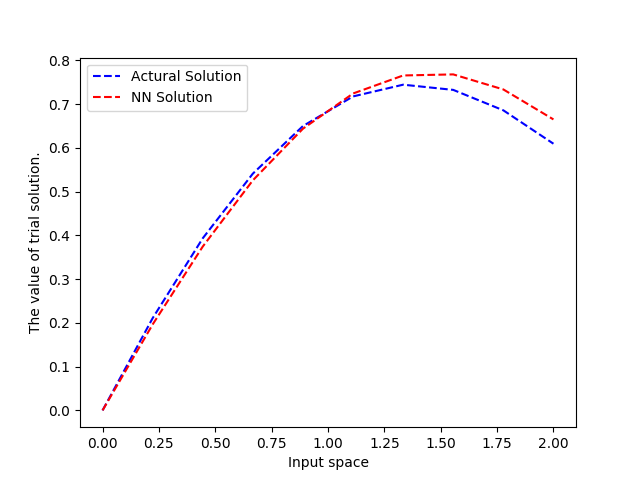
\includegraphics[width=0.5\textwidth]{ode_3.png}
	\caption{The actual and computed solution in problem 1.3. }
	\label{fig:trial_ode3}
\end{figure}

\section{Schematic of the Algorithm}

This section provides the formulation for differential equation to adjust in order to solve 
\[\frac{du}{dx}(x) \in \mathbb{R}, x \in \mathbb{R}^N, n\in\{0,1, \dots , N\}\]
by NN.

\subsection{Formulation}

The proposed approach is illustrated in terms of the following general differential equation:
\begin{equation}\label{eq:original_error}
G(\bar{x},u (\bar{x}),\bigtriangledown \hat{u} (\bar{x}), \bigtriangledown \hat{u} (\bar{x})^2, \dots) = 0, x \in \Omega
\end{equation}
\medskip \noindent
subject to certain boundary conditions (B.Cs),  where $ \bar{x}=(x_1, \dots , x_n) \in \mathbf{R}^n, \Omega \subset \mathbf{R}$ and $\hat{u}$ is the trial solution employs a neural network and $\Omega$ denotes the definition of domain.
\begin{equation}\label{eq:trial_solution}
u_{trial}(x,p) = \hat{u}(x) + F(x,\bar{u}(\bar{x}))
\end{equation}

$\hat{u}(x)$ is the initial conditions(I.C.) which is set to be $\hat{u}(0) = u (0)$ and contains no adjustable parameters.
The scalar-value function $F(x)$ is chosen so as not to contribute to BC.
$\bar{u}(w,v,\bar{x})$ is the output forward neural network(NN).
In order to be solved by NN, we transform (\ref{eq:original_error}) to the  following system of equations:
%\begin{equation}\label{eq:3}
%G(x_i,u (x_i),\bigtriangledown u (x_i), \bigtriangledown u (x_i)^2) = 0, \forall %x_i \in D, \forall i = 1 \dots m
%\end{equation}
\begin{equation}\label{eq:total_error_sum}
E(w,v;\bar{u}(\bar{x})) = \min \sum_{i=1}^{m} G(x_i,\hat{u} (\bar{x}),\bigtriangledown \hat{u} (\bar{x}), \bigtriangledown \hat{u} (\bar{x})^2, \dots) ^2, \forall x_i \in \Omega, \forall i = 1 \dots N
\end{equation}

If $u_{trial}(x,p)$ denotes the trial solution, $u_{trial}(x,p)$ will minimize the related error of (\ref{eq:total_error_sum}). 

%\medskip \noindent
%\textbf{Below is the outline of the NN for solving ODE: }
%\begin{itemize}
%	\item Input $x_i$: The number of equidistant points for (\ref{eq:total_error_sum}) in $x\in D, \forall i = 1 \dots N$. For example, if the $D={x^{(i)} \in D; i = 1, \dots , 10}$, the $E_{\text{error}}$ is trained by discretizing  $10$ equidistant points in $[0,1]$.
%	\item Hidden layer $h$: Each unit in the layer corresponds to the discrete time step with sigmoid activation function in (\ref{eq:activation}).
%	\item Output $Q_{i}$: The output is used to measure the trial solution in (\ref{eq:forward_output}).
%\end{itemize}


\section{Stochastic Gradient Descent}
Lagaris\cite{lagaris} had proved that Broyden–Fletcher–Goldfarb–Shanno (BFGS) algorithm method is quadraticly convergent and has demonstrated excellent performance at computing the gradient of the error.
Therefore, quasi-Newton BFGS algorithm was used to minimize the loss function in our model.



\subsection{ODE}
\subsubsection{First Order ODE}
We consider the first order ODE:
\[\frac{du}{dx}(x)=f(x,u)\]
We discretinize our domain $[0,1]$ into n grids and obtain input vector $x_i$, $1 \leq i \leq N$ where i denotes the single input unit in discretenized domain.
We apply activation function to obtain the output of hidden unit. A popular choice for choosing activation function is the sigmoid function.
\begin{equation}\label{eq:sigmoid}
\sigma(y) = \frac{1}{1+e^{y}}
\end{equation}
The output of hidden units given by activation function is mapped from 0 to 1.
\begin{equation}\label{eq:hidden_unit}
H_{j}(x_i) =  \sigma (w_{ij}*x_i), 1 \leq j \leq M
\end{equation}

\medspace \noindent
The output forward propogation of NN is:
\begin{equation}\label{eq:output_ode}
Q_i (w,v,x_i)=  \sum_{j=1}^{M} \textit{v}_{j}H(x_i)
\end{equation}
\medspace \noindent
Figure \ref{fig:nn_ode_struct} expresses the diagram of NN with one hidden layer looking for the parameters for trial solution in ode and pde. This example only has one hidden layer. After we get the output for whole $x_{i}$, $i \in \{0, \dots , n\}$ via NN, we obtain the sum of error quantity.

\begin{figure}
	\centering
	\includegraphics[width=0.4\textwidth]{nn_ode_struct.png}
	\caption{The diagram of Neural Network for computing the parameters of trial solution in ode $Q_{i}(x_i,p)$ with one hidden layer. }
	\label{fig:nn_ode_struct}
\end{figure}

\begin{equation}\label{eq:total_error_ode}
\begin{aligned}
E(w,v,\bar{x})= \sum_{i=1}^{N}\sum_{j=1}^{M} \{ \frac{d u_{trial}}{dx}(x_i)-f(x_{i}, u_{trial}(x_i))\}^{2}
\end{aligned}
\end{equation}

\medskip \noindent
where p is the parameters in NN and $f(x_i,u_{trial}(x_i))$ is the value of $\frac{d}{dx}u$.
In the case of one dimension ode, we obtain the value after we shift all the items except for $\frac{d}{dx}u$ to the right side.

\medskip \noindent
We optimize the parameters of NN by minimizing the total error quantity in (\ref{eq:total_error_ode}) from $E_i, i \in \{1 \dots n\}, h \in \{1 \dots M\}$.
\begin{equation}\label{eq:weight_ode_v}
\frac{\partial E}{\partial v_{j}}(w,v) = \sum_{i=1}^{N} \frac{\partial E}{\partial Q_{i}}(w,v)  \frac{\partial Q_{i}}{\partial v_{j}}
\end{equation}
\begin{equation}\label{eq:weight_ode_w}
\frac{\partial E}{\partial w_{ij}}(w,v) = \sum_{i=1}^{N} \frac{\partial E}{\partial Q_{i}}(w,v) \frac{\partial Q_{i}}{\partial w_{ij}}
\end{equation}
where h is the number of hidden unit in each hidden layer, $1 \leq h \leq H$

\begin{equation}\label{eq:weight_ode_Ev}
\frac{\partial E}{\partial Q_{i}}(w,v;\bar{u}_i) = 2\left(\{\frac{\partial u_{trial}}{\partial x}(x_i)-f(x_{i}, u_{trial}(x_i))\}\right)
\end{equation}
\medskip \noindent
To calculate the (\ref{eq:weight_ode_Ev}). We need to differentiate the trial solution $u_{trial}(x_i)$:
\begin{equation}\label{eq: ode_trial_x}
\frac{\partial u_{trial} }{\partial x}(x_i) = \frac{d u}{dx}(0) + \frac{d Q_{i}}{dx}(w,v,x_i) + x\frac{d Q_{i}}{dx}(w,v,x_i)
\end{equation}
These equations reduce to
\begin{equation}\label{eq:x_ode_Psix}
\frac{\partial u_{trial} }{\partial x}(x_i) = Q_{i}(x,p) + \sum_{i=1}^{N}\sum_{h=1}^{M} \textit{v}_{j} w_{ij} \sigma (w_{ij}x_{i})_{j}
\end{equation}
Using (\ref{eq:x_ode_Psix}) and $f(x_{i}, u_{trial}(x_i))$, the gradient of $Q_{i}$ is:
\begin{equation}\label{eq:partial_NV}
\frac{\partial Q}{\partial v} (w,v,\bar{x})= \sum_{j=1}^{M} \sum_{i=1}^{N}\sigma (w_{ij}x_{i})
\end{equation}
\medspace \noindent
We compute the gradient of $E(w,v;\bar{u})$ with respect to input to hidden weight by using (\ref{eq:weight_ode_v})-(\ref{eq:partial_NV}) and get:
\begin{equation} \label{eq:weight_ode_ow}
\frac{\partial Q}{\partial w} (w,v,\bar{x})= \sum_{h}^{M} \sum_{i=1}^{N} (\sigma(x_{i}w_{ij}))'x_i
\end{equation}
\medskip \noindent
Finally, we obtain the gradient of total error quantity with respect to the network weights in (\ref{eq:weight_ode_v}) and (\ref{eq:weight_ode_w}). The network weight can be easily updated as:
\begin{equation}
\begin{aligned}
w_{ij}^{(k+1)} = w_{ij}^{(k)} - \gamma_{k}*\frac{\partial E_i}{\partial w_{ij}} \\
v_{j}^{(k+1)} = v_{j}^{(k)} - \gamma_{k}*\frac{\partial E_i}{\partial v_{j}}
\end{aligned}
\end{equation}

\subsubsection{Kth Order ODE}

 The different thing between the multiple order ODE and first order ODE is the total of error sum quantity and the trial solution.  We use second order ODE for example to illustrate the way to find the solution of kth order ODE where k is larger than 1.

\medspace \noindent
We consider the second order ODE:
\[\frac{d^2}{dx^2}u(x)=f(x,u,\frac{d}{dx}u)\]

\medspace \noindent
The sum of error quantity to be minimized becomes:

\begin{equation}\label{eq:total_error_ode2}
E(w,v;\bar{u}(\bar{x})) =\sum_{i=1}^{N} \{ \frac{d^{2} u_{trial}}{dx^2}(x_i)-f(x_{i}, u_{trial}(x_i), \frac{d}{dx}u_{trial}(x_i)) \}^{2}
\end{equation}
\medspace \noindent
The trial solution is written as:
\begin{equation}\label{eq: ode2_trial_x}
u_{trial}(x) = u(0)(1-x)+ u(1)x+x(1-x)\bar{u}(\bar{x})
\end{equation}
\medspace \noindent
To obtain the $\frac{d^2}{dx^2}u(x_i)$ in \ref{eq:total_error_ode2}, we differentiate the trial solution $u_{trial}(x_i)$ from (\ref{eq: ode2_trial_x}) to obtain the one and second order of $u_{trial}(x_i)$.

\begin{equation} \label{eq:ode2_trial_dx}
\frac{d u_{trial}}{dx} = -u_{analytic}(0) + u_{analytic}(1) + \bar{u}(\bar{x}) +x\frac{\partial \bar{u}}{\partial x}(\bar{x}) - 2x\bar{u}(\bar{x}) - x^{2}\frac{\partial \bar{u}}{\partial x}(\bar{x})
\end{equation}

\begin{equation} \label{eq:ode2_trial_dxx}
\frac{d^{2}}{dx^{2}}u_{trial}  = -2\bar{u}(w,v,\bar{x}) + 2\frac{\partial \bar{u} }{\partial x}(w,v,\bar{x}) -4x\frac{\partial \bar{u}}{\partial x}(w,v,\bar{x}) + x\frac{\partial^{2} \bar{u}}{\partial x^{2}}(w,v,\bar{x}) - x^{2}\frac{\partial^{2}  \bar{u}}{\partial^{2} x}(w,v,\bar{x})
\end{equation}

After we computing the derivative of sum of total error quantity with respect to $Q(x,p)$, we can follow the formulation for computing gradient of the feedforward NN's $Q(x,p)$ with respect to the network weights using (\ref{eq:weight_ode_v})-(\ref{eq:partial_NV}) in section 3.1.1.

\subsection{PDE}

\subsubsection{Two-Dimension PDE}
Solving the kth order PDE by NN is similar with solving first order PDE.  We consider the Poisson equation:
\begin{equation}
\frac{\partial^{2} u }{\partial x^2}(x,y)+ \frac{\partial^{2} u }{\partial y^2}(x,y) = f(x,y).
\end{equation}
with $x \in [0,1], y \in [0,1]$. 
The error quantity to be minimized is given by:
\begin{equation}
E(w,v;\bar{u}(\bar{x})) = \sum_{i} \left \{ 
\frac{\partial^{2} u_{trial} }{\partial x^2}(x,y)+ \frac{\partial^{2} u_{trial} }{\partial y^2}(x,y)-
f\left( x,y,u(x_i),\frac{\partial u_{trial}}{\partial x}, \frac{\partial u_{trial}}{\partial x}\right)
 \right \}^2.
\end{equation}
The form of trial solution is based on the types of Boundary conditions encountered in the solution of partial differential equations. For a Dirichlet BC, the trial solution is:
\begin{equation}
u_{trial}(x,y) = A(x,y) + x(1-x)y(1-y)\bar{u}(\bar{x},\bar{y}).
\end{equation}
where $A(x, y)$ is chosen so as to satisfy the BC.
\begin{equation} \label{eq:pde_dir}
A(x, y) = (1-x)u_a(0,y)+xu_a(1,y)+(1-y)\{u_a(x,0)-[(1-x)u_a(0,0)+xu_a(1,0)]\}+y\{u_a(x,1)-[(1-x)u_a(0,1)+xu_a(1,1)]\}
\end{equation}

\medskip\noindent
Let $F(a,y)=(1-a)u_a(x_1,y)+au_a(x_N,y)$. We can reduce  (\ref{eq:pde_dir}) to :

\begin{equation}
A(x,y)=F(\bar{x},y)+F(y,Y(\bar{x},y_1),Y(\bar{x},y_N))
\end{equation}

where 
\[Y = u_a(x,y)-F(x,u_a(x_1,y),u_a(x_N,y))\]
Since $x\in[0,1],y\in[0,1]$,
\[Y(x,y_1) = u_a(x,0)-F(x,u_a(0,0),u_a(1,0))\]
\[Y(x,y_N) = u_a(x,1)-F(x,u_a(0,1),u_a(1,1))\]

\medskip \noindent
For a mixed boundary condition, the trial solution is written as:

\begin{equation}
	u_{trial}(x,y) = B(x,y) + x(1-x)y\left[\bar{u}(\bar{x},\bar{y})-\bar{u}(\bar{x},1)-\frac{\partial}{\partial y}\bar{u}(\bar{x},1)\right]
\end{equation}
$B(x, y)$ is again chosen so as to satisfy the BCs.
\begin{equation}\label{eq:pde_mixed}
B(x, y) = (1-x)u_a(0,y)+xu_a(1,y)+u_a(x,0)−[(1-x)u_a(0,0)+xu_a(1,0)]+y\left \{ \frac{d}{dy}u_a(x,1)-\left[(1-x)\frac{d}{dy}u_a(0,1)+x\frac{d}{dy}u_a(1,1)\right] \right \}
\end{equation}

We can reduce (\ref{eq:pde_mixed}) to:

\begin{equation}
B(x,y)=F(\bar{x},y)+Y(\bar{x},y_1)+Y(\bar{x},y_N)'
\end{equation}

where 

\[{Y}'=\frac{d u}{dy}(x,1)-{F}'( \bar{x},y_N) = \frac{d u}{dy}(x,1)\]

where ${F}'=(1-x)\frac{\partial u_a}{\partial}(x_1,y)+xu_a(x_N,y)$

\medskip \noindent
Figure \ref{fig:nn_pde_struct} illustrate the way to compute the parameters by NN for trial solution in two-dimensional problem. We denote the feedforward function as $Q(w,v,x_i,y_i)$.

\begin{figure}
	\centering
	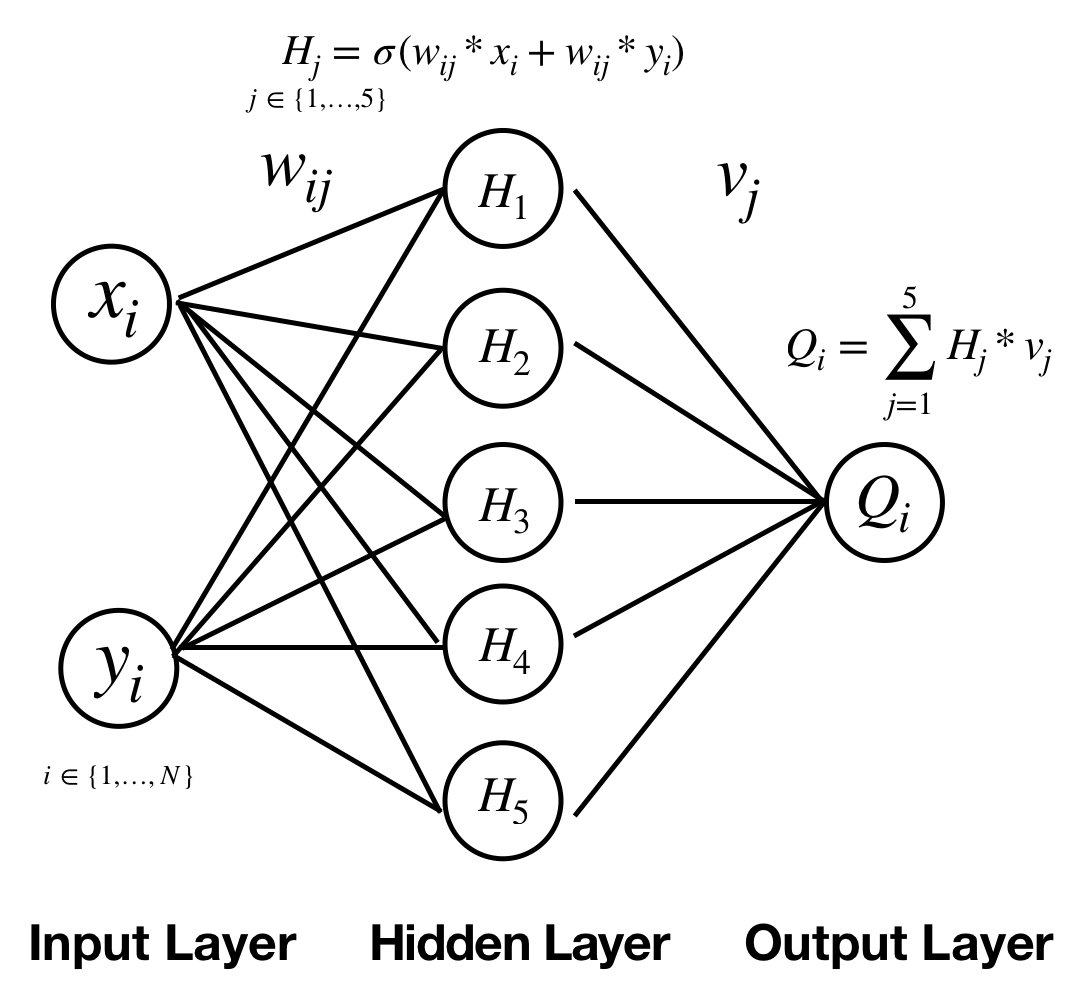
\includegraphics[width=0.4\textwidth]{nn_pde_struct.png}
	\caption{The diagram of Neural Network for computing the parameters of trial solution in pde $Q_{i}(x_i,y_i,p)$ with one hidden layer. }
	\label{fig:nn_pde_struct}
\end{figure}


\section{Convergence Method}

Because we did not apply activation function to the output unit of NN, the value of output does not converge. Therefore, in order to make the output stable, we set the condition that if
\begin{equation}\label{eq:converge}
| u_{trial}(x_N) - BC| \leq \varepsilon
\end{equation}
\medspace \noindent
and the number of iteration is over 500, then the iteration stops. In (\ref{eq:converge}), we set $BC=u_{analytic}(x_N)$ and $\varepsilon=e^{-3}$.







\section{Relative Work}

Weinan\cite{weinan} combines backward stochastic differential equation(BSDE) with NN to solve PDE.
Trial solution is for the stochastic control problem.
The stochastic process with continuous sample paths which satisfy that for all $t \in [0,T]$.
\begin{equation}
Y_t = g(\xi + W_T) + \int_{t}^{T}f(Y_s,Z_s)ds - \int_{t}^{T}\langle  Z_s,dW_s \rangle
\end{equation}
The nonlinear PDE is related to BSDE in a sense that for all $t \in [0,T]$ it holds that
\begin{equation}
Y_t = u(t,\xi + W_t) \in \mathbf{R}, \ \ \ \ Z_t=(\bigtriangledown_{x}u)(t,\xi + W_t) \in \mathbf{R}
\end{equation}
To approximate the trial solution, they can be computed approximately by employing the policy Z.

%\subsubsection{Neural Network with Backward Stochastic Differential Equation}
%They formulate the PDE problem as a form of Stochastic Differential Equation and approximate $\triangledown_x u(t,x_t)$ by neural network.

%\medskip \noindent
%Let $\hat{u_t}=u_{trial}(t,x)$ be a dynamic $\hat{u}$ starts at time t in x.  The range of time horizon $T$ corresponds to the index of domain $\Omega$ in our method. 
%\medskip \noindent
%By Ito formula 
%\[d\hat{u_t} = -f(t,x_t,y_t, \triangledown_x u(t,x_t))dt + \triangledown_x u(x_i)\sigma(x_t)dW_{t}\]
%where $W$ denotes Brownian motion. 

%\medskip\noindent
%If $u_{trial}(t,x_t)$ solve the equation, we obtain for $\hat{u_t}=u(t,x_t)$ and $Z_{t}=\triangledown_x u(x_i)\sigma(x_t)dW_{t}$.
%\[d\hat{u_t}=-f(t,x_t,y_t, \triangledown_x u(t,x_t))dt + Z_{t}dW_{t}\]
%\medskip \noindent
%Therefore, the way to approximate $u_{trial}$ in their paper is:

%\begin{equation}
%\begin{aligned}
%Y_{t_{n+1}} &= Y_{t_{n}} + \int_{t_n}^{t_{n+1}}f(Y_s,Z_s)ds - \int_{t}^{T}\langle  Z_s,dW_s \rangle \\
%&\approx  Y_{t_{n}} - f(Y_{t_{n}},Z_{t_{n}})((t_{n+1})-(t_{n})) + Z_{t_{n}}dW_{t_{n}}((t_{n+1})-t_{n})
%\end{aligned}
%\end{equation}



%\bibliographystyle{unsrt}
%\bibliography{nn_pde}
\begin{thebibliography}{9}
	\bibitem{lagaris}
I. E. Lagaris, A. Likas and D. I. Fotiadis,
\textit{Artifial Neural Networks for Solving Ordinary and Partial Differential Equations},
IEEE Transaction on Neural Networks, vol. 9, No. 5, September 1998

\bibitem{chiaramonte}
M. M. Chiaramonte and M. Kiener,
\textit{Solving differential equations using neural networks}

\bibitem{weinan}
E, Weinan, Han, Jiequn and Jentzen, Arnulf,
\textit{Deep Learning-Based Numerical Methods for High-Dimensional Parabolic Partial Differential Equations and Backward Stochastic Differential Equations},
A. Commun. Math. Stat. (2017) 5: 349.
\end{thebibliography}

\end{document}
